\Variant{01.03.2026 (2-smena)}
\QQ{1}{$\overline{8962ab}$ körinişdagi son $12$ ga qoldiqsiz bölinsa, $a\cdot b$ ning eng katta qiymatini toping.
\Opts{$24$}{$48$}{$36$}{$30$}}
\QQ{2}{Hisoblang ($[a]$ — $a$ sonining butun qismi, $\{a\}$ — kasr qismi):
\[\bigl\{3\cdot[\lg5]+5\cdot\{\lg0{,}1\}-7[\ln3]\bigr\}\]
\Opts{$0$}{$7$}{$\dfrac{21}{48}$}{$\dfrac9{28}$}}
\QQ{3}{$A$ punktdan $B$ punktga piyoda yölga çiqdi. Oradan $3$ soat ötgaç, uning ortidan velosipedçi yölga çiqdi. Velosipedçi yölning yarmiga yetganida piyodani quvib ötdi. Agar velosipedçining tezligi piyodaning tezligidan $4$ marta katta bölsa, piyoda $A$ dan $B$ gaça bölgan masofani neça soatda bosib ötadi?
\Opts{$6$}{$8$}{$10$}{$12$}}
\QQ{4}{Tadbirkor bitta köylak va bitta şimni sotib oldi. Agar u köylakni $40\%$ ga, şimni $45\%$ ga qimmatlatib sotsa, $215\,000$ söm foyda köradi. Agar aksinça, köylakni $45\%$ ga, şimni $40\%$ ga qimmatlatib sotsa, $210\,000$ söm foyda köradi. Köylakning tannarxini toping.
\Opts{$180\,000$}{$200\,000$}{$250\,000$}{$300\,000$}}
\QQ{5}{Hisoblang:
\[\left(1+\left(2-\left(3+(4-1)^{-1}\right)^{-1}\right)^{-1}\right)^{-1}\]
\Opts{$\dfrac{27}{17}$}{$\dfrac{10}{17}$}{$\dfrac{17}{27}$}{$\dfrac3{10}$}}
\QQ{6}{Hisoblang:
\[\left(9{,}4\cdot\sqrt[3]{6^2\sqrt6}-3{,}4\sqrt{6\sqrt[3]{6^2}}\right)^{\frac6{11}}\]
\Opts{$36$}{$6$}{$\sqrt[6]6$}{$1$}}
\QQ{7}{Hisoblang:
\[\sqrt[3]{26+15\sqrt3}+\sqrt[3]{26-15\sqrt3}\]
\Opts{$2$}{$3$}{$4$}{$5$}}
\QQ{8}{$(a_n)$ arifmetik progressiyada $a_2=2a_1$ va $a_{10}=20$ bölsa, $S_6-S_5$ ni hisoblang.
\Opts{$10$}{$12$}{$14$}{$16$}}
\QQ{9}{$\{a_n\}$ arifmetik progressiya ($d\ne0$) va $\{b_n\}$ geometrik progressiya berilgan. Agar $a_1+a_2+a_3+\ldots+a_n=820$, $b_1+b_2+b_3=217$, $b_1=a_2$, $b_2=a_9$ va $b_3=a_{44}$ bölsa, $n$ ni toping.
\Opts{$18$}{$20$}{$22$}{$24$}}
\QQ{10}{Agar $\dfrac{x-2}y=1$ va $y\ne-1$ bölsa, $\dfrac{2x+4y+2}{x+y}$ ning qiymatini toping.
\Opts{$0$}{$2$}{$3$}{$6$}}
\QQ{11}{Soddalaştiring:
\[\frac1{a+\frac1{b+\frac1c}}:\frac1{a+\frac1b}-\frac1{b(abc+a+c)}\]
\Opts{$\dfrac1a$}{$\dfrac1b$}{$\dfrac ab$}{$1$}}
\QQ{12}{Hisoblang:
\[\frac{\sin11^\circ-\sin49^\circ}{1-2\cos^254{,}5^\circ}\]
\Opts{$\sqrt3$}{$-\sqrt3$}{$\dfrac{\sqrt3}3$}{$-\dfrac{\sqrt3}3$}}
\QQ{13}{Tenglama $\left[-\dfrac\pi2;\,\pi\right]$ oraliqda neçta yeçimga ega?
\[\sqrt3\sin^2x+\sin^22x=\frac{\sqrt3}2-\frac12-\sqrt3\cos2x\]
\Opts{$2$}{$3$}{$0$}{$1$}}
\QQ{14}{Tengsizlikni yeçing:
\[(0{,}75)^{\frac{x^2+x-8}{x+1}}>0{,}6\cdot(1{,}25)^{x-\frac8{x+1}}\]
\Opts{$(-3;\,-1)\cup(3;\,\infty)$}{$(-\infty;\,-3)\cup(-1;\,3)$}{$(-3;\,-1)\cup(-1;\,3)$}{$(-\infty;\,-3)\cup(3;\,\infty)$}}
\QQ{15}{Tengsizlikni neçta butun son qanoatlantiradi?
\[\log_{0{,}5}\log_2\log_{x-1}9>0\]
\Opts{$7$}{$5$}{$6$}{çeksiz köp}}
\QQ{16}{Tenglama neçta haqiqiy ildizga ega?
\[\left|x^2-5x-6\right|+\left|7+6x-x^2\right|=x+1\]
\Opts{$2$}{$3$}{yeçimga ega emas}{çeksiz köp yeçimga ega}}
\QQ{17}{Tenglama neçta haqiqiy ildizga ega?
\[8x^3-6x^2+3x-1=0\]
\Opts{$1$}{$2$}{$3$}{yeçimga ega emas}}
\QQ{18}{Tengsizlikni yeçing:
\[\frac1{x+1}+\frac2{x+3}-\frac3{x+2}>0\]
\Opts{$(-3;\,-2)\cup(-1;\,\infty)$}{$(-\infty;\,-3)\cup(-2;\,-1)\cup(1;\,\infty)$}{$(-3;\,-2)\cup(-1;\,1)$}{$(-3;\,-2)\cup(-2;\,-1)\cup(-1;\,1)$}}
\QQ{19}{Tengsizlikni qanoatlantiruvçi butun sonlar yiğindisini toping.
\[\left(2x^2-x-2\right)^2<\left(x^2+5x+4\right)^2\]
\Opts{$15$}{$21$}{$28$}{$18$}}
\QQ{20}{Rasmda $f(x)=ax^3+bx^2+cx+d$ funksiyaning grafigi tasvirlangan. Rasmdagi maʼlumotlar asosida $f(-3)$ ni toping.
\qfig{\begin{tikzpicture}[scale=0.6,font=\small]
\draw[-{Stealth[length=4pt]}] (-3,0)--(3.2,0) node[right] {$x$}; \draw[-{Stealth[length=4pt]}] (0,-2.6)--(0,4.6) node[left] {$y$};
\draw[thick,domain=-2.3:2.45,samples=80] plot (\x,{0.45*(\x*\x*\x-4*\x)});
\draw[dashed] (-1,0)--(-1,1.35)--(0,1.35);
\node[right] at (0,1.35) {$3$}; \node[below left] at (-2,0) {$-2$}; \node[below] at (-1,0) {$-1$}; \node[below right] at (2,0) {$2$}; \node[below left] at (0,0) {$O$};
\end{tikzpicture}}
\Opts{$-14$}{$-13$}{$-15$}{$-16$}}
\QQ{21}{Aniqmas integralni hisoblang:
\[\int\frac x{\sqrt{3x+1}}\,dx\]
\Opts{$\dfrac29\cdot\left(\dfrac13(3x+1)^{\frac12}+(3x+1)^{\frac32}\right)+C$}{$\dfrac29\cdot\left(\dfrac13(3x+1)^{\frac12}-(3x+1)^{\frac32}\right)+C$}{$\dfrac29\cdot\left(\dfrac13(3x+1)^{\frac32}+(3x+1)^{\frac12}\right)+C$}{$\dfrac29\cdot\left(\dfrac13(3x+1)^{\frac32}-(3x+1)^{\frac12}\right)+C$}}
\QQ{22}{Agar $f(x)=\left|\ln x-\log_{\sin x}\cos x\right|$ bölsa, $f'\!\left(\dfrac\pi4\right)$ ni toping.
\Opts{$\dfrac4\pi-\dfrac4{\ln2}$}{$-\dfrac4\pi+\dfrac4{\ln2}$}{$-\dfrac4\pi-\dfrac4{\ln2}$}{$\dfrac4\pi+\dfrac4{\ln2}$}}
\QQ{23}{Uçburçakning eng katta tomoni $8$ ga, qolgan tomonlari esa $3x-4$ va $2x+1$ ga teng. Agar uçburçakning tomonlari butun sonlardan iborat bölsa, uçburçak perimetrini toping.
\qfig{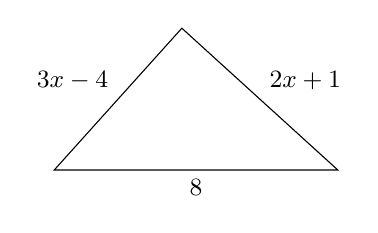
\begin{tikzpicture}[scale=0.45,font=\small]
\draw (0,0)--(8,0)--(3.6,4)--cycle;
\node[above left] at (1.8,2) {$3x-4$}; \node[above right] at (5.8,2) {$2x+1$}; \node[below] at (4,0) {$8$};
\end{tikzpicture}}
\Opts{$16$}{$17$}{$18$}{$20$}}
\QQ{24}{Agar $f(x)$ noldan farqli juft funksiya va $g(x)$ noldan farqli toq funksiya bölsa, quyidagilardan neçtasi toq funksiya böladi?
\par\smallskip I. $y_1=f(x)\cdot g(x)$;\qquad II. $y_2=f(x)+g(x)$;\qquad III. $y_3=\dfrac{f(x)}{g(x)}$.
\Opts{$0$}{$1$}{$2$}{$3$}}
\QQ{25}{$ABC$ muntazam uçburçakka radiuslari teng bölgan $O_1$, $O_2$ va $O_3$ markazli aylanalar rasmdagidek içki çizilgan. $ABC$ uçburçak yuzining $O_1O_2O_3$ uçburçak yuziga nisbatini toping.
\qfig{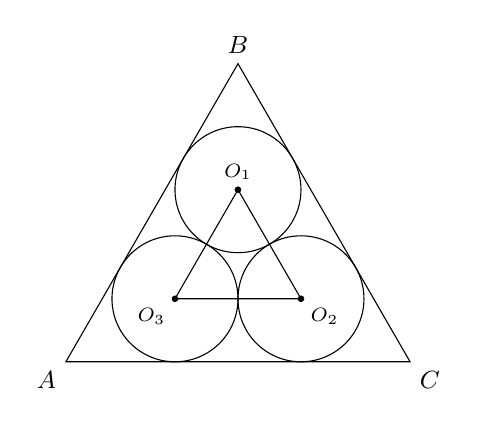
\begin{tikzpicture}[scale=0.8,font=\small]
\coordinate (A) at (0,0); \coordinate (C) at (5.464,0); \coordinate (B) at (2.732,4.732);
\coordinate (O3) at (1.732,1); \coordinate (O2) at (3.732,1); \coordinate (O1) at (2.732,2.732);
\draw (A)--(B)--(C)--cycle; \foreach \p in {O1,O2,O3} {\draw (\p) circle (1); \fill (\p) circle (1.5pt);}
\draw (O1)--(O2)--(O3)--cycle;
\node[below left] at (A) {$A$}; \node[above] at (B) {$B$}; \node[below right] at (C) {$C$};
\node[above,font=\scriptsize] at (O1) {$O_1$}; \node[below right,font=\scriptsize] at (O2) {$O_2$}; \node[below left,font=\scriptsize] at (O3) {$O_3$};
\end{tikzpicture}}
\Opts{$8$}{$4+2\sqrt3$}{$4$}{$8+2\sqrt3$}}
\QQ{26}{$ABC$ teng yonli uçburçakda $AB=BC$ va $AC=64$. Uçburçakka radiusi $16$ ga teng bölgan aylana içki çizilgan. Radiusi $r$ ga teng bölgan kiçik aylana $AB$ va $BC$ tomonlarga hamda katta aylanaga urinadi. $r$ ni toping.
\qfig{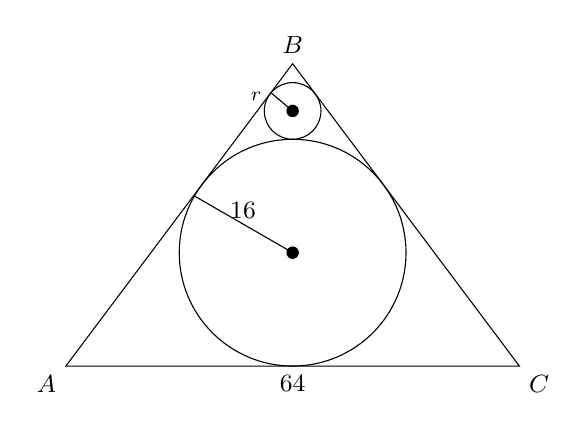
\begin{tikzpicture}[scale=0.09,font=\small]
\coordinate (A) at (0,0); \coordinate (C) at (64,0); \coordinate (B) at (32,42.67);
\draw (A)--(B)--(C)--cycle; \draw (32,16) circle (16); \draw (32,36) circle (4);
\fill (32,16) circle (25pt); \fill (32,36) circle (25pt);
\draw (32,16)--++(150:16); \draw (32,36)--++(140:4);
\node[below left] at (A) {$A$}; \node[above] at (B) {$B$}; \node[below right] at (C) {$C$}; \node[below] at (32,0) {$64$};
\node[above] at (25,19.5) {$16$}; \node[left,font=\scriptsize] at (29,38) {$r$};
\end{tikzpicture}}
\Opts{$2$}{$4$}{$6$}{$12$}}
\QQ{27}{Çizmada $ABCD$ trapetsiyaning ($BC\parallel AD$) $AC$ va $BD$ diagonallari $O$ nuqtada kesişadi. Agar $BOC$ va $AOD$ uçburçaklarning yuzalari mos ravişda $2$ va $8$ ga teng bölsa, böyalgan soha yuzini toping.
\qfig{\begin{tikzpicture}[scale=0.45,font=\small]
\coordinate (A) at (0,0); \coordinate (D) at (10,0); \coordinate (B) at (1,4); \coordinate (C) at (6,4); \coordinate (O) at (4,2.667);
\fill[qfill] (A)--(B)--(O)--cycle;
\draw (A)--(B)--(C)--(D)--cycle; \draw (A)--(C); \draw (B)--(D);
\node[below left] at (A) {$A$}; \node[above left] at (B) {$B$}; \node[above right] at (C) {$C$}; \node[below right] at (D) {$D$}; \node[below=2pt] at (O) {$O$};
\end{tikzpicture}}
\Opts{$4$}{$8$}{$5$}{$6$}}
\QQ{28}{Rasmda $ABCD$ kvadrat, $CED$ va $BCP$ muntazam uçburçaklar tasvirlangan. Şunga köra $\angle DKE$ burçakni toping.
\qfig{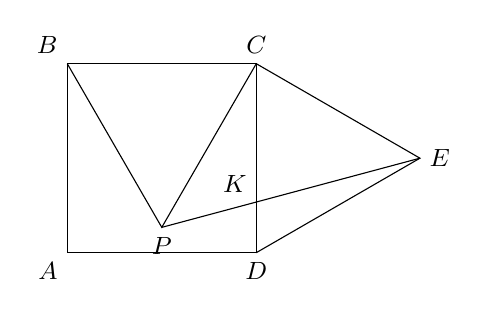
\begin{tikzpicture}[scale=0.6,font=\small]
\coordinate (A) at (0,0); \coordinate (B) at (0,4); \coordinate (C) at (4,4); \coordinate (D) at (4,0); \coordinate (P) at (2,0.536); \coordinate (E) at (7.464,2); \coordinate (K) at (4,1.072);
\draw (A)--(B)--(C)--(D)--cycle; \draw (B)--(P)--(C); \draw (C)--(E)--(D); \draw (P)--(E);
\node[below left] at (A) {$A$}; \node[above left] at (B) {$B$}; \node[above] at (C) {$C$}; \node[below] at (D) {$D$}; \node[right] at (E) {$E$}; \node[below] at (P) {$P$}; \node[above left] at (K) {$K$};
\end{tikzpicture}}
\Opts{$100^\circ$}{$75^\circ$}{$120^\circ$}{$105^\circ$}}
\QQ{29}{$A(-2;\,5;\,-4)$, $B(-2;\,7;\,-1)$ va $C(4;\,7;\,2)$ nuqtalar berilgan. $ABC$ uçburçakda $AC$ tomonga $BD$ mediana ötkazilgan. $\sin\angle CBD$ ni toping.
\Opts{$\dfrac{\sqrt7}5$}{$-\dfrac{\sqrt7}5$}{$\dfrac{3\sqrt2}5$}{$-\dfrac{3\sqrt2}5$}}
\QQ{30}{$ABC$ teng yonli töğri burçakli uçburçakning ($\angle C=90^\circ$) $BC$ kateti $\alpha$ tekislikda yotadi. $AC$ kateti $\alpha$ tekislik bilan $45^\circ$ li burçak taşkil qiladi. $AB$ gipotenuza va $\alpha$ tekislik orasidagi burçakni toping.
\Opts{$30^\circ$}{$45^\circ$}{$\arctg2$}{$60^\circ$}}
\QQ{31}{Sinfda jami $25$ nafar öquvçi bor. Ulardan $9$ nafari biologiya tögaragiga, $8$ nafari kimyo tögaragiga qatnaşadi. $10$ nafar öquvçi esa heç qaysi tögarakka qatnaşmaydi. Ikkala tögarakka ham qatnaşadigan öquvçilar sonini toping.
\Opts{$2$}{$3$}{$4$}{$5$}}
\QQ{32}{Ikkita kesişmaydigan töğri çiziqdan $3$ ta va $4$ ta nuqta olingan. Şu nuqtalarni tutaştirişdan neçta uçburçak hosil qiliş mumkin?
\Opts{$15$}{$24$}{$27$}{$30$}}
\QQ{33}{\Moslash{Töğri prizmaning asosi teng yonli $ABCD$ trapetsiyadan ($BC\parallel AD$) iborat va prizmaga şar içki çiziş mumkin. Trapetsiya asoslari $8$ va $18$ ga teng. Prizmaning $AA_1D_1D$ va $BB_1C_1C$ yon yoqlariga $KK_1N_1N$ va $LL_1M_1M$ parallel kesimlar ötkazilgan.
\par\centering\begin{tikzpicture}[scale=0.95,font=\scriptsize]
\coordinate (A) at (0,0.64); \coordinate (B) at (2.16,1.45); \coordinate (C) at (4.1,1.166); \coordinate (D) at (4.36,0);
\coordinate (K) at (1.08,1.045); \coordinate (N) at (4.23,0.583); \coordinate (L) at (1.495,1.2); \coordinate (M) at (4.18,0.807);
\def\H{3.3}
\foreach \p in {A,B,C,D,K,N,L,M} \coordinate (\p1) at ($(\p)+(0,\H)$);
\fill[qfill,opacity=0.6] (K)--(N)--(N1)--(K1)--cycle; \fill[qfill,opacity=0.6] (L)--(M)--(M1)--(L1)--cycle;
\draw (A)--(D)--(D1)--(A1)--cycle; \draw (A1)--(B1)--(C1)--(D1); \draw (A1)--(C1); \draw (B1)--(D1);
\draw[dashed] (A)--(B)--(C)--(D); \draw[dashed] (B)--(B1); \draw[dashed] (C)--(C1); \draw[dashed] (A)--(C); \draw[dashed] (B)--(D);
\draw[dashed] (K)--(N); \draw[dashed] (L)--(M); \draw (K1)--(N1); \draw (L1)--(M1);
\draw[dashed] (K)--(K1); \draw[dashed] (L)--(L1); \draw[dashed] (M)--(M1); \draw[dashed] (N)--(N1);
\node[left] at (A) {$A$}; \node[above] at (B) {$B$}; \node[above right] at (C) {$C$}; \node[below right] at (D) {$D$};
\node[below] at (K) {$K$}; \node[above left] at (L) {$L$}; \node[right] at (M) {$M$}; \node[right] at (N) {$N$};
\node[left] at (A1) {$A_1$}; \node[above] at (B1) {$B_1$}; \node[above right] at (C1) {$C_1$}; \node[right] at (D1) {$D_1$};
\node[above left] at (K1) {$K_1$}; \node[above] at (L1) {$L_1$}; \node[right] at (M1) {$M_1$}; \node[right] at ($(N1)+(0,-0.12)$) {$N_1$};
\end{tikzpicture}}{A) $12\sqrt{313}$\par B) $132\dfrac{12}{13}$\par C) $156\sqrt{13}$\par D) $256\dfrac{11}{13}$\par E) $156$\par F) $6\sqrt{313}$}{Prizmaning $AA_1C_1C$ diagonal kesimi yuzini toping.}{Trapetsiyaning diagonallari kesişiş nuqtasidan ötuvçi $LL_1M_1M$ kesim yuzini toping.}{Trapetsiyaning örta çiziği bilan bir töğri çiziqda yotuvçi $KK_1N_1N$ kesim yuzini toping.}}
\QQ{36}{$r$, $s$, $t$ haqiqiy sonlar $f(x)=x^3+ax^2+bx+1$ funksiyaning nollari, $r^2$, $s^2$, $t^2$ haqiqiy sonlar esa $g(x)=x^3+mx^2+nx+p$ funksiyaning nollari va $g(-1)=-5$ bölsa,
\AB{$n-m-p$ ning qiymatini toping.}{$(a-1)^2+(b-1)^2$ ning qiymatini toping.}}
\QQ{37}{Tenglamani yeçing:
\[\sin^4x+2\sin^22x=9\cos^4x\]
\AB{Tenglama $\left[-\dfrac\pi2;\,\dfrac{5\pi}2\right]$ oraliqda neçta ildizga ega?}{Tenglamaning $[-\pi;\,\pi]$ oraliqdagi ildizlari yiğindisini toping.}}
\QQ{38}{$y=f(x)$ kvadrat funksiya uçun $f(0)=2$ bölsa,
\AB{$f(x+5)=f(x)+x+1$ tenglik örinli bölsa, $f(2025)$ ning qiymatini toping.}{$f(x-9)=f(x)+x-3$ tenglik örinli bölsa, $f(2025)$ ning qiymatini toping.}}
\QQ{39}{$y=x^2-6x+12$ kvadrat funksiya berilgan. Parabolaga ötkazilgan urinma $y=2x+1$ töğri çiziq bilan kesişmaydi.
\qfig{\begin{tikzpicture}[scale=0.42,font=\small]
\draw[-{Stealth[length=4pt]}] (-2,0)--(7.5,0) node[right] {$x$}; \draw[-{Stealth[length=4pt]}] (0,-2.5)--(0,8.4) node[left] {$y$};
\draw[thick,domain=0.7:5.3,samples=60] plot (\x,{\x*\x-6*\x+12}) node[right] {$y=x^2-6x+12$};
\draw[thick] (-0.8,-0.6)--(3.2,7.4) node[right] {$y=2x+1$};
\draw[thick] (-1.2,4.4)--(2.3,-2.6) node[right] {$y=-2x+2$};
\node[below left] at (0,0) {$O$};
\end{tikzpicture}}
\AB{Urinmaning parabolaga uriniş nuqtasi ordinatasini toping.}{$y=x^2-6x+12$ funksiya grafigidan $A$ nuqta, $y=-2x+2$ funksiya grafigidan $B$ nuqta olingan. $A$ va $B$ nuqtalar orasidagi mumkin bölgan eng qisqa masofani toping.}}
\QQ{40}{$y_1=x^2$ va $y_2=\sqrt x$ funksiyalar berilgan.
\qfig{\begin{tikzpicture}[scale=2.2,font=\small]
\fill[qfill] plot[domain=0:1,samples=50] (\x,{sqrt(\x)}) -- plot[domain=1:0,samples=40] (\x,{\x*\x}) -- cycle;
\draw[-{Stealth[length=4pt]}] (-0.2,0)--(1.5,0) node[right] {$x$}; \draw[-{Stealth[length=4pt]}] (0,-0.2)--(0,1.5) node[left] {$y$};
\draw[thick,domain=0:1.4,samples=60] plot (\x,{sqrt(\x)}) node[right] {$y_2=\sqrt x$};
\draw[thick,domain=-0.3:1.2,samples=60] plot (\x,{\x*\x}) node[above] {$y_1=x^2$};
\node[below left] at (0,0) {$O$};
\end{tikzpicture}}
\AB{$y_1$ va $y_2$ funksiyalar grafiklari bilan çegaralangan soha yuzini toping.}{Şu sohani $Ox$ öqi atrofida $360^\circ$ ga aylantirişdan hosil bölgan jism hajmini toping ($\pi\approx3$ deb olinsin).}}
\QQ{41}{$ABC$ uçburçakda $\angle A>\angle B>\angle C$. $AC$ va $BC$ tomonlarga ötkazilgan örta perpendikulyarlar mos ravişda $B$ va $A$ burçak bissektrisalari bilan $E$ va $F$ nuqtalarda kesişadi, $O$ — uçburçakka taşqi çizilgan aylana markazi. Agar $\angle AFO=5^\circ$, $\angle BEO=10^\circ$ va $AC=3$ bölsa,
\qfig{\begin{tikzpicture}[scale=1.3,font=\small]
\coordinate (A) at (0,0); \coordinate (C) at (3,0); \coordinate (B) at (0.908,2.494); \coordinate (O) at (1.5,0.866); \coordinate (E) at (1.5,-0.866); \coordinate (F) at (2.827,1.98); \coordinate (M) at (1.954,1.247);
\draw (A)--(B)--(C)--cycle; \draw (A)--(F); \draw (B)--(E); \draw (E)--(1.5,0.866); \draw (O)--(F);
\draw (1.5,0)++(0,0.12)--++(0.12,0)--++(0,-0.12);
\draw ($(M)!0.12cm!(C)$)--($(M)!0.12cm!(C)!0.12cm!90:(C)$)--($(M)!0.12cm!90:(C)$);
\fill (O) circle (1pt);
\node[below left] at (A) {$A$}; \node[above] at (B) {$B$}; \node[below right] at (C) {$C$}; \node[left] at (O) {$O$}; \node[below] at (E) {$E$}; \node[right] at (F) {$F$};
\end{tikzpicture}}
\AB{$\angle ACB$ burçak kattaligini toping.}{$OF$ ning qiymatini toping.}}
\QQ{42}{$ABCD$ trapetsiyaning kiçik asosi $BC=56$. Trapetsiyaga taşqi çizilgan aylanadagi $E$ nuqtadan $DC$ tomonga parallel urinma va trapetsiya asoslariga parallel $EF$ vatar ötkazilgan. Agar $EF=70$ va aylana radiusi $14\sqrt7$ ga teng bölsa,
\qfig{\begin{tikzpicture}[scale=0.055,font=\small]
\coordinate (O) at (0,0); \coordinate (A) at (-37,-1.732); \coordinate (D) at (37,-1.732); \coordinate (B) at (-28,24.25); \coordinate (C) at (28,24.25); \coordinate (E) at (35,12.12); \coordinate (F) at (-35,12.12);
\draw (O) circle (37.04); \draw (A)--(B)--(C)--(D)--cycle; \draw (F)--(E); \draw (O)--(E);
\draw ($(E)+(-0.3273*16,0.9449*16)$)--($(E)-(-0.3273*16,0.9449*16)$); \fill (O) circle (25pt);
\node[left] at (A) {$A$}; \node[above left] at (B) {$B$}; \node[above right] at (C) {$C$}; \node[below right] at (D) {$D$}; \node[right] at (E) {$E$}; \node[left] at (F) {$F$}; \node[below] at (O) {$O$};
\node[above] at (0,24.25) {$56$}; \node[above] at (-8,12.12) {$70$}; \node[below] at (14,5) {$14\sqrt7$};
\end{tikzpicture}}
\AB{Trapetsiya diagonalini toping.}{Trapetsiya yuzini toping.}}
\QQ{43}{Muntazam sakkizburçakka aylana içki çizilgan, aylanaga esa muntazam oltiburçak içki çizilgan.
\qfig{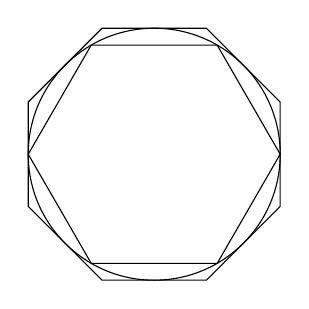
\begin{tikzpicture}[scale=1.6]
\draw (0,0) circle (1);
\draw (22.5:1.0824)--(67.5:1.0824)--(112.5:1.0824)--(157.5:1.0824)--(202.5:1.0824)--(247.5:1.0824)--(292.5:1.0824)--(337.5:1.0824)--cycle;
\draw (0:1)--(60:1)--(120:1)--(180:1)--(240:1)--(300:1)--cycle;
\end{tikzpicture}}
\AB{Aylana markazidan muntazam oltiburçak tomonigaça bölgan masofaning muntazam sakkizburçak tomonigaça bölgan masofaga nisbatini toping.}{Muntazam oltiburçak yuzining muntazam sakkizburçak yuziga nisbatini toping.}}
\QQ{44}{Muntazam törtburçakli kesik piramidaga şar içki çizilgan. Kesik piramidaning töla sirti $312$ ga teng. Kesik piramida katta asosi yuzining kiçik asosi yuziga nisbati $9$ ga teng.
\AB{Kesik piramida hajmini toping.}{Şar hajmini toping.}}
\QQ{45}{Yon qirralari $2$ ga teng bölgan muntazam törtburçakli piramida berilgan. Agar piramida eng katta hajmga ega bölsa,
\AB{Piramida asosining yuzini toping.}{Piramida hajmini toping.}}
\Javoblar{B A B B C B C B B C D B B B B D A C B C D B D C B B A D A A A D A B E}{\OK{36}{$4$}{$5$}\OK{37}{$6$}{$0$}\OK{38}{$409\,457$}{$-228\,148$}\OK{39}{$4$}{$\dfrac{6\sqrt5}5$}\OK{40}{$\dfrac13$}{$0{,}9$}\OK{41}{$50^\circ$}{$\sqrt3$}\OK{42}{$70$}{$975\sqrt3$}\OK{43}{$\dfrac{\sqrt3}2$}{$\dfrac{3\sqrt3(\sqrt2+1)}{16}$}\OK{44}{$312$}{$36\pi$}\OK{45}{$\dfrac{16}3$}{$\dfrac{32\sqrt3}{27}$}}
